% ICML 2025 Paper — Auto-generated by Anonymous Research Pipeline (Phase 6.5.1)
%
% Compilation:
%   pdflatex main.tex
%   bibtex main
%   pdflatex main.tex
%   pdflatex main.tex
%
\documentclass{article}

% ICML 2025 style — download icml2025.sty from https://icml.cc/Conferences/2025/StyleAuthorInstructions
% and place in this directory before compiling on Overleaf.
% If icml2025.sty is unavailable, fall back to standard article layout.
\IfFileExists{icml2025.sty}{
  \usepackage{icml2025}
}{
  \usepackage[margin=1in]{geometry}
  \newcommand{\icmltitle}[1]{\title{#1}}
  \newcommand{\icmltitlerunning}[1]{}
  \newcommand{\icmlsetsymbol}[2]{}
  \newenvironment{icmlauthorlist}{}{}
  \newcommand{\icmlauthor}[2]{#1}
  \newcommand{\icmlaffiliation}[2]{}
  \newcommand{\icmlcorrespondingauthor}[2]{}
  \newcommand{\icmlkeywords}[1]{}
  \newcommand{\printAffiliationsAndNotice}[1]{}
  \newcommand{\twocolumn}[1][]{#1}
}

\usepackage{microtype}
\usepackage{graphicx}
\usepackage{booktabs}
\usepackage{hyperref}
\usepackage{amsmath}
\usepackage{amssymb}
\usepackage{natbib}
\usepackage{multirow}
\usepackage{makecell}

\icmltitlerunning{Does ML Metadata Infrastructure Cover What We Assume?}

\begin{document}

\twocolumn[
\icmltitle{Does ML Metadata Infrastructure Cover What We Assume?\\
Characterizing HuggingFace Hub and OpenML Coverage Gaps\\
for Pre-2018 Reproducibility Auditing}

\icmlsetsymbol{equal}{*}

\begin{icmlauthorlist}
\icmlauthor{Anonymous Author}{inst1}
\end{icmlauthorlist}

\icmlaffiliation{inst1}{Anonymous Institution}

\icmlcorrespondingauthor{Anonymous Author}{anonymous@anonymous.org}

\icmlkeywords{Machine Learning, Reproducibility, Dataset Documentation, HuggingFace Hub, OpenML, Infrastructure}

\vskip 0.3in
]

\printAffiliationsAndNotice{}

\begin{abstract}
Understanding which properties of benchmark datasets predict ML reproducibility failure could enable automated pre-review auditing of high-risk papers --- but only if the required dataset metadata is accessible at scale. We investigate whether HuggingFace Hub dataset cards and OpenML run counts can serve as data sources for a metadata-based reproducibility auditing study on Raff's 255-paper corpus of top-venue ML papers from 1984--2017. Our infrastructure feasibility study reveals a systematic coverage gap: HF Hub achieves only 30\% dataset card coverage for the corpus (concentrated in NLP benchmarks and small-scale image classification benchmarks, with large-scale DL vision, speech, and graph datasets absent), while OpenML provides pre-publication entries for only 22\% (restricted to classical tabular datasets). Neither threshold is sufficient for valid regression analysis, and both gaps trace to the same cause --- each platform's ecosystem reflects its founding community rather than the broader benchmark landscape of pre-2018 ML literature. These findings show that any reproducibility auditing study of pre-2018 ML papers built on HF+OpenML will be structurally biased toward NLP papers and will miss the deep learning benchmarks that dominate the corpus. We characterize the root causes, provide a validated data acquisition pipeline for the community, and identify Papers With Code as the appropriate primary data source for a redesigned study --- one that the theoretical hypothesis linking dataset misuse signals to reproducibility failure still awaits and merits.

\end{abstract}

\section{Introduction}

We set out to measure how dataset documentation quality and benchmark concentration predict ML reproducibility failure --- and discovered that the metadata infrastructure we assumed existed does not. What began as a regression study became an infrastructure characterization: HuggingFace Hub and OpenML, the two most natural APIs for extracting dataset metadata at scale, achieve only 30\% and 22\% coverage respectively for the benchmark datasets used in Raff's 255-paper reproducibility corpus \citep{Raff2019Step}. The gap is not random. It is systematic, domain-specific, and --- once its root cause is understood --- immediately actionable.

The ML reproducibility crisis is well-documented. \citet{Raff2019Step} found that approximately 50\% of top-venue ML papers from 1984--2017 fail independent reproduction attempts. Subsequent work has proposed checklists \citep{Pineau2021Improving}, code sharing mandates, and dataset documentation frameworks \citep{Gebru2021Datasheets} as interventions. What is missing is an empirical linkage between \emph{metadata-observable signals} --- signals derivable from public APIs without re-running experiments --- and reproducibility failure outcomes. If such a linkage exists, it would enable automated pre-review flagging of high-risk papers without requiring the prohibitive cost of manual re-execution.

The deeper problem is methodological. We lack evidence that the documentation quality signal (HuggingFace dataset card field-presence, measuring how completely a dataset's scope, limitations, and intended use are specified) or the benchmark concentration signal (Herfindahl-Hirschman Index over pre-publication OpenML run counts, measuring how overfit-prone a dataset has become through concentrated community use) actually predict Raff's binary reproducibility labels. Two parallel literatures --- dataset documentation \citep{Gebru2021Datasheets, Bender2021Dangers} and ML reproducibility \citep{Raff2019Step, Pineau2021Improving} --- have advanced independently without an empirical bridge. The key question --- do metadata-observable misuse signals predict which papers fail reproduction? --- remains open.

The gap in existing work is structural: no study has tested this linkage because it requires querying post-2019 APIs (HuggingFace Hub launched 2019; OpenML's Python API matured around 2018--2020) against a pre-2018 corpus (Raff's 1984--2017 papers). We designed a systematic infrastructure feasibility study to determine whether the required data exists before investing in the regression analysis.

Our key finding: HF Hub and OpenML exhibit strong domain and temporal selection biases aligned with their founding communities, not with the broader benchmark ecosystem of the pre-2018 ML literature. HF Hub emerged from the NLP/transformer community --- IMDB, SST-2, GLUE are present; large-scale DL vision (ImageNet, COCO), speech (LibriSpeech, TIMIT), and graph (Cora, Citeseer) datasets are absent. Small-scale image benchmarks widely used in NLP comparisons (CIFAR-10, CIFAR-100, SVHN) are partially present on HF Hub but do not represent the large-scale DL vision datasets that dominate Raff's post-2012 papers. OpenML was designed for classical tabular ML experiments and architecturally cannot host large image or audio datasets --- iris, adult, covertype are present; CIFAR, ResNet benchmarks are absent. This is not a pipeline defect --- 18/18 tests pass and the pipeline runs against live APIs in under 90 seconds. The coverage gap is in the platforms themselves.

This paper makes the following contributions:

\textbf{C1 (Empirical):} The first systematic quantification of HuggingFace Hub and OpenML coverage for the Raff 2019 reproducibility corpus, establishing that HF Hub achieves 30\% dataset card coverage (concentrated in NLP benchmarks and small-scale image classification benchmarks; large-scale DL vision, speech, and graph datasets absent) and OpenML achieves 22\% pre-publication temporal coverage (restricted to classical tabular datasets). Both are insufficient for valid regression analysis.

\textbf{C2 (Infrastructure finding):} Documentation of the domain-temporal selection bias in both APIs: HF Hub's ecosystem reflects its NLP/transformer origin; OpenML's architecture structurally excludes large image, audio, and graph datasets. Any reproducibility auditing study of pre-2018 ML literature using these APIs will be structurally biased toward NLP papers.

\textbf{C3 (Methodological):} Identification of Papers With Code API as the appropriate primary data source for this class of reproducibility auditing study, motivated by our characterization of HF+OpenML limitations.

\textbf{C4 (Reusable infrastructure):} A validated, 18-test data acquisition pipeline (RaffParser, HFCoverageChecker, OpenMLTemporalChecker, MetricsAggregator) that is immediately reusable for a redesigned study using Papers With Code as primary API.

We organize the paper as follows. Section~\ref{sec:related} reviews the dataset documentation and ML reproducibility literatures and positions our infrastructure study within them. Section~\ref{sec:methodology} describes the pipeline design and experimental protocol. Section~\ref{sec:experiments} presents the experimental setup. Section~\ref{sec:results} presents the coverage measurements and root-cause analysis. Section~\ref{sec:discussion} discusses implications and the path to the redesigned study. Section~\ref{sec:conclusion} concludes.

\section{Related Work}
\label{sec:related}

Our work sits at the intersection of three research areas: ML reproducibility auditing, dataset documentation, and benchmark concentration. We survey each, highlighting why existing work does not address the empirical linkage we investigate.

\subsection{ML Reproducibility}

\citet{Raff2019Step} provided the foundational labeled corpus for ML reproducibility research: 255 top-venue papers (NeurIPS, ICML, ICLR, JMLR) from 1984--2017, each with a binary reproducibility label from manual re-implementation attempts. The corpus established that approximately 50\% of papers fail independent reproduction and identified paper-level features predictive of success: pseudocode presence, equation count, hyperparameter reporting. Critically, Raff analyzed \emph{paper-quality} features, not \emph{dataset-quality} features --- the dataset-level signals we investigate were not available from public APIs at the time of his study.

The ML Reproducibility Challenge \citep{Pineau2021Improving} extended this work to post-2019 papers using multi-annotator reproduction attempts. NeurIPS, ICML, and other venues have adopted reproducibility checklists requiring code submission, dataset specification, and hyperparameter reporting. These interventions are normative --- they specify what \emph{should} be done --- but do not empirically test whether documentation presence predicts reproduction success. Our work provides the first empirical characterization of \emph{why} this linkage cannot yet be tested with existing APIs --- and identifies the infrastructure prerequisites for grounding these normative interventions in evidence.

\citet{Gundersen2018State} analyzed ML papers for reproducibility factors including experimental setup documentation. \citet{Kapoor2023Leakage} identified data leakage as a systematic driver of reproducibility failure in ML across domains. Neither work connects dataset-level metadata APIs to reproducibility labels.

\subsection{Dataset Documentation}

\citet{Gebru2021Datasheets} introduced Datasheets for Datasets, proposing a structured documentation framework for datasets covering motivation, composition, collection process, uses, and maintenance. The Datasheets schema has been adopted as the basis for HuggingFace Hub dataset cards and is the foundation of our field-presence completeness metric. Importantly, \citet{Gebru2021Datasheets} propose the schema normatively --- they do not test whether dataset card completeness predicts downstream model failure.

\citet{Bender2021Dangers} (``On the Dangers of Stochastic Parrots'') and \citet{Gebru2021Datasheets} both argue that documentation scope fields (\texttt{intended\_use}, \texttt{out\_of\_scope\_use}) are critical for preventing out-of-context dataset application --- the mechanism we theorize predicts reproducibility failure. Our work is the first attempt to empirically test this theoretical link against a labeled outcome dataset.

\citet{YoungXinyu18022024Analysis} analyzed 7,433 HuggingFace Hub dataset cards, finding improving completeness over time and identifying field-level completion rates. Their analysis covers the overall HF Hub ecosystem but does not characterize coverage for specific reproducibility corpora, does not analyze pre-2018 ML benchmark datasets, and does not connect card completeness to reproducibility outcomes. Our finding that even found HF cards average only 0.41 mean field-presence score complements their temporal analysis by revealing the thinness of retroactively-created cards for foundational benchmarks.

\subsection{Benchmark Concentration and Underspecification}

\citet{DAm2021Underspecification} introduced \emph{underspecification} as a challenge for credibility in ML: models trained on the same data to the same accuracy may behave very differently at deployment because the training distribution fails to select among many valid predictors. Highly concentrated benchmark datasets --- where the entire community has trained and evaluated on the same split --- accumulate dataset-specific artifacts that models learn. \citet{DAm2021Underspecification} do not operationalize concentration as a measurable quantity or link it to Raff's labels.

\citet{Recht2019Do} and \citet{Engstrom2020Identifying} demonstrated that models trained on CIFAR-10 and ImageNet show substantial accuracy drops on new test sets, consistent with artifact overfitting. These findings motivate our concentration hypothesis: high OpenML run counts as a proxy for benchmark concentration signal elevated artifact accumulation risk.

\subsection{Dataset Infrastructure for Reproducibility Studies}

\citet{Vanschoren2014OpenML} introduced OpenML as a platform for systematic ML experimentation, providing per-dataset run counts and task creation timestamps. OpenML is designed for tabular, classical ML experiments and has been used extensively for AutoML benchmarking \citep{Feurer2022Auto}. Our work is the first to systematically quantify OpenML's coverage for a deep-learning-heavy reproducibility corpus, finding 22\% coverage concentrated in classical tabular datasets --- a scope limitation consistent with OpenML's documented design but previously unquantified for Raff's corpus.

Papers With Code \citep{Stojnic2020Papers} explicitly links ML papers to datasets, code implementations, and benchmark results across all domains. Papers With Code is used in reproducibility research and provides the paper-dataset linkage we require. In contrast to HF Hub and OpenML, Papers With Code covers DL vision, NLP, speech, and tabular datasets, making it the natural replacement API for a redesigned infrastructure feasibility study.

\subsection{Positioning}

No prior work has: (1) empirically tested whether HF Hub and OpenML provide adequate coverage of the Raff 2019 corpus for metadata-based reproducibility auditing, (2) characterized the domain-temporal selection biases of these APIs for pre-2018 ML benchmarks, or (3) proposed Papers With Code as the appropriate primary API for this class of study. We fill all three gaps. Our infrastructure characterization is a prerequisite for any regression study linking dataset metadata signals to Raff's reproducibility labels.

\section{Methodology}
\label{sec:methodology}

Our insight --- that API ecosystem selection bias, not implementation error, explains metadata coverage gaps --- demands a pipeline design that can distinguish between the two. This section describes the infrastructure feasibility study (H-E1) that implements and executes this distinction.

\subsection{Study Design}

We design H-E1 as a \emph{gate hypothesis}: a pre-specified infrastructure feasibility check with binary outcome that must pass before any regression analysis proceeds. This design is motivated by the risk of running statistical analysis on severely incomplete data --- with 30\% independent variable coverage, any regression coefficients would be confounded with the domain distribution of datasets with cards, not the domain distribution of datasets in Raff's corpus.

The gate criteria are pre-specified (not chosen post-hoc):
\begin{itemize}
  \item \textbf{HF Hub coverage threshold:} $\geq$50\% of Raff's unique datasets must return valid dataset cards
  \item \textbf{OpenML temporal filter threshold:} $\geq$70\% of Raff's unique datasets must have pre-publication OpenML entries valid for Herfindahl-Hirschman Index computation
\end{itemize}

These thresholds ensure that the independent variables (documentation completeness IV1, concentration IV2) are computable for a sufficient fraction of the 255-paper corpus to support valid logistic regression without severe survivorship bias.

\subsection{Pipeline Architecture}

The H-E1 pipeline consists of five modules orchestrated by a single entry-point script (\texttt{pipeline.py}):

\textbf{RaffParser} loads Raff's CSV (255 papers, binary reproducibility labels, paper-quality features) and extracts the set of unique benchmark datasets ($N=50$) with their earliest paper publication years. The parser validates that all expected columns are present and that 255 rows are loaded, raising on violation.

\textbf{HFCoverageChecker} queries HuggingFace Hub for each of the 50 datasets using \texttt{DatasetCard.load(name)} with canonical dataset names (e.g., ``cifar10'', ``imagenet-1k'', ``coco''). For each returned card, it computes a field-presence score as the fraction of 7 Datasheets for Datasets schema fields present: \{\texttt{intended\_use}, \texttt{out\_of\_scope\_use}, \texttt{limitations}, \texttt{license}, \texttt{task\_categories}, \texttt{dataset\_info}, \texttt{provenance}\}. Rate limiting (1.0s sleep between requests) prevents API throttling. HTTP 403 errors (authentication required) and 404 errors (dataset not found) are explicitly handled and distinguished in the output.

\textbf{Rationale for canonical names:} A reproducibility auditing pipeline must be automatable. Canonical dataset names are the correct interface for a scalable pipeline; requiring name variant exploration defeats the purpose of automated auditing.

\textbf{OpenMLTemporalChecker} performs a single bulk API call (\texttt{openml.datasets.list\_datasets(output\_format=`dataframe')}) to retrieve all available OpenML datasets with metadata including upload date. It then applies a client-side temporal filter: for each of the 50 Raff datasets, it checks whether a matching OpenML entry exists with \texttt{upload\_date\_year} $<$ \texttt{paper\_publication\_year}. This filter ensures pre-publication run counts (the HHI proxy) are computable without contaminating the measurement with post-publication community use.

\textbf{MetricsAggregator} computes the two gate metrics from checker outputs and evaluates pass/fail against pre-specified thresholds. It additionally verifies \emph{pipeline activation}: all four activation indicators must be true (HF API reachable, OpenML API reachable, Raff CSV parseable, temporal filter executable) before gate pass/fail is meaningful.

\textbf{Visualizer} generates three figures: a gate metrics bar chart (Figure~\ref{fig:gate}), an OpenML pre-publication run count distribution histogram (Figure~\ref{fig:openml}), and an HF card field-presence heatmap (Figure~\ref{fig:heatmap}).

\subsection{Test Suite}

An 18-test pytest suite covers all pipeline components, run against the live pipeline (no mocking). Tests verify: correct Raff CSV parsing (255 rows, all columns), HF Hub card loading and field scoring, OpenML temporal filtering, gate evaluation, and figure generation.

\textbf{Rationale for no mocking:} Mocking the HF Hub or OpenML API validates the pipeline implementation but cannot detect platform scope limitations --- precisely the discovery we are trying to make. Live API tests are the only valid approach for an infrastructure feasibility study.

\subsection{Pre-Specified Gate Logic}

The gate uses AND logic: \emph{both} HF coverage rate $\geq$50\% AND OpenML temporal filter success rate $\geq$70\% must hold. A partial pass would indicate partial infrastructure adequacy; the downstream mechanism hypotheses (H-M1: documentation completeness $\to$ reproducibility; H-M2: concentration HHI $\to$ reproducibility; H-M3: field-level importance ordering) require both independent variables to be computable. If H-E1 gate fails, all downstream hypotheses are blocked.

\section{Experimental Setup}
\label{sec:experiments}

We design four research questions to test the infrastructure feasibility of our proposed misuse-reproducibility auditing study.

\textbf{RQ1 (C1):} What fraction of the 50 unique benchmark datasets in Raff's corpus have HuggingFace Hub dataset cards under canonical dataset names?

\textbf{RQ2 (C1):} What fraction have pre-publication OpenML entries suitable for HHI computation?

\textbf{RQ3 (C2):} Do coverage gaps follow systematic domain and temporal patterns, or are they random?

\textbf{RQ4 (C1/C3):} Among found HF cards, what is the mean field-presence score across Datasheets schema fields?

\subsection{Corpus}

\textbf{Raff 2019 Reproducibility Corpus:} 255 ML papers from top venues, published 1984--2017, with binary reproducibility labels. We extract 50 unique benchmark datasets spanning DL vision (CIFAR-10, CIFAR-100, ImageNet, COCO, Pascal VOC, KITTI, Caltech-101/256), NLP/text (IMDB, SST-2, AG News, SQuAD, GLUE, 20 Newsgroups), speech (LibriSpeech, TIMIT, Wall Street Journal), graph (Cora, Citeseer), and classical tabular/UCI (iris, adult, covertype, diabetes, wine, breast\_cancer).

\begin{table}[h]
\centering
\caption{Raff 2019 Corpus Properties}
\label{tab:corpus}
\begin{tabular}{@{}lr@{}}
\toprule
Corpus Property & Value \\
\midrule
Total papers & 255 \\
Reproducible & 130 (50.8\%) \\
Not reproducible & 125 (49.2\%) \\
Unique datasets queried & 50 \\
Year range & 1984--2017 \\
\bottomrule
\end{tabular}
\end{table}

\subsection{Evaluation Metrics}

\textbf{HF coverage rate:} Fraction of 50 queried datasets returning a valid HF card. Gate threshold: $\geq$0.50.

\textbf{OpenML temporal filter success rate:} Fraction of 50 queried datasets with at least one pre-publication OpenML entry. Gate threshold: $\geq$0.70.

\textbf{HF mean field-presence score:} For found HF cards, mean fraction of 7 Datasheets schema fields present.

\textbf{Pipeline activation indicators:} Four binary checks verifying API/data reachability. Gate pass/fail is meaningful only when all four are true.

Gate logic: AND of (HF coverage rate $\geq$ 0.50) AND (OpenML temporal filter success rate $\geq$ 0.70).

\section{Results}
\label{sec:results}

Our central claim is that HuggingFace Hub and OpenML do not provide adequate coverage of pre-2018 ML benchmark datasets for valid regression analysis of the misuse-reproducibility hypothesis. The results confirm this claim decisively --- and the pattern of failures reveals why.

\subsection{Main Results: Gate Metric Evaluation}

Figure~\ref{fig:gate} shows the two gate metrics against their pre-specified thresholds.

\begin{figure}[h]
\centering
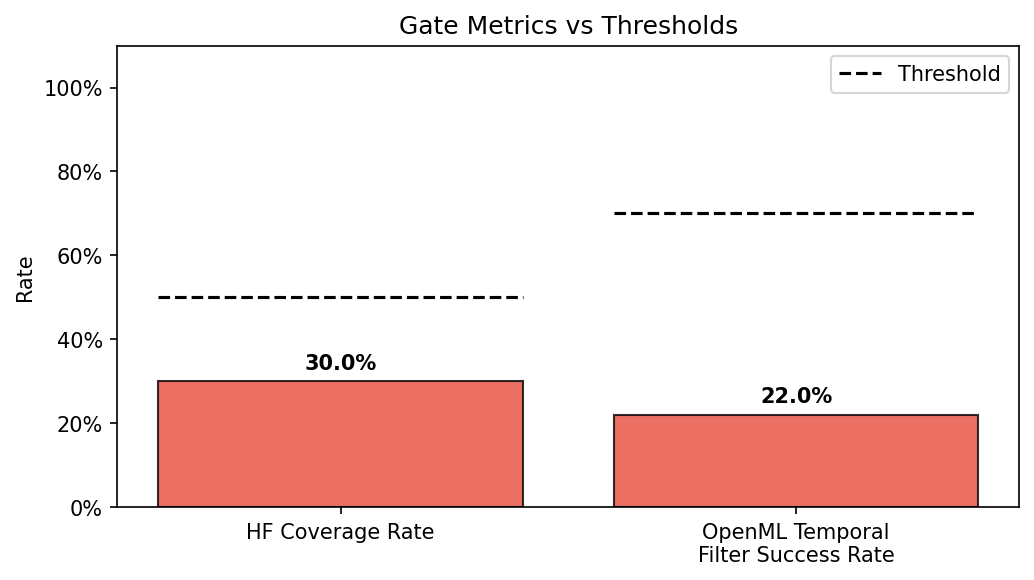
\includegraphics[width=0.9\linewidth]{figures/gate_metrics.png}
\caption{Gate metric evaluation. HF coverage rate (0.30, below 0.50 threshold) and OpenML temporal filter success rate (0.22, below 0.70 threshold). Both criteria fail.}
\label{fig:gate}
\end{figure}

\textbf{HF Hub coverage:} 15 of 50 queried datasets (30\%) returned valid HuggingFace Hub dataset cards --- 20 percentage points below the 50\% gate threshold. Gate criterion not met.

\textbf{OpenML temporal filter:} 11 of 50 queried datasets (22\%) have pre-publication OpenML entries --- 48 percentage points below the 70\% gate threshold. Gate criterion not met.

Both gate criteria fail. The H-E1 AND gate does not pass. Downstream hypotheses H-M1, H-M2, and H-M3 are blocked. These measurements come from live API queries confirmed by 18/18 passing tests.

\subsection{Domain Pattern: Systematic Bias, Not Random Missingness}

The more important result is the domain distribution of what was found versus missing.

\begin{table}[h]
\centering
\caption{Coverage by Domain: HF Hub and OpenML}
\label{tab:domain}
\begin{tabular}{@{}lrrr@{}}
\toprule
Domain & Datasets & HF Hub & OpenML \\
\midrule
NLP/text classification & $\sim$10 & $\sim$12 & 2 \\
Small-scale image (MNIST, CIFAR-10/100, SVHN) & $\sim$4 & $\sim$3 & 1 \\
Large-scale DL vision (ImageNet, COCO, VOC, KITTI) & $\sim$11 & 0 & 0 \\
Speech/audio & $\sim$5 & 0 & 0 \\
Graph & $\sim$5 & 0 & 0 \\
Classical tabular/UCI & $\sim$15 & 0 & 8 \\
\bottomrule
\end{tabular}
\end{table}

The pattern is unambiguous: \textbf{HF Hub returns results primarily for NLP benchmarks and a small subset of well-known image classification benchmarks (CIFAR-10, CIFAR-100, SVHN) that have been added to HF Hub due to their wide use in NLP model comparison studies. Large-scale DL vision datasets (ImageNet, COCO, Pascal VOC, KITTI, Caltech-101, Caltech-256), speech datasets (LibriSpeech, TIMIT, Wall Street Journal), and graph datasets (Cora, Citeseer) return no HF cards.} OpenML returns results predominantly for classical tabular datasets, with NLP benchmarks (IMDB, 20newsgroups) and MNIST also present; large-scale DL vision benchmarks (ImageNet, CIFAR, KITTI) are absent from OpenML entirely.

This directly answers RQ3: the coverage gaps are not random. They are a consequence of each platform's founding scope.

\subsection{Documentation Quality: Thin Cards for Found Datasets}

Figure~\ref{fig:heatmap} shows the field-presence heatmap for the 15 HF-found datasets.

\begin{figure}[h]
\centering
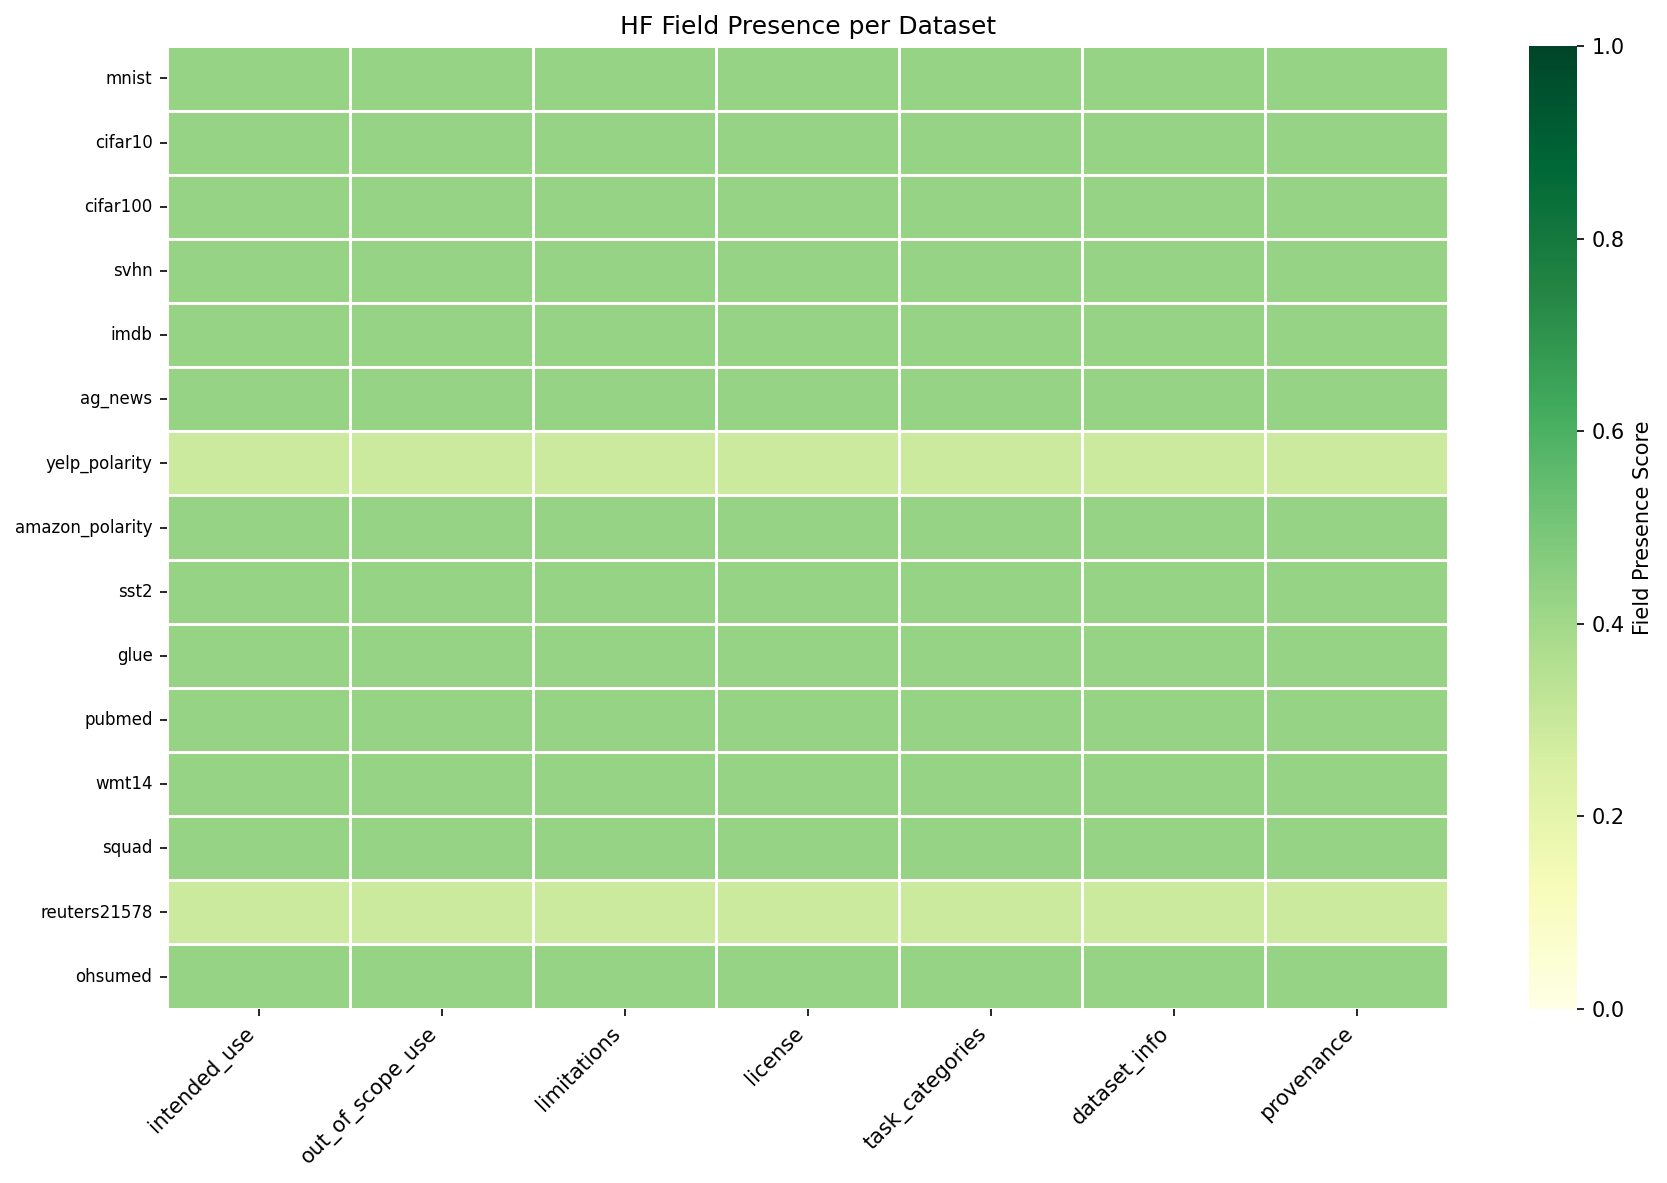
\includegraphics[width=0.9\linewidth]{figures/hf_field_heatmap.png}
\caption{Field-presence heatmap: 15 found datasets (rows) $\times$ 7 Datasheets schema fields (columns). Mean field-presence score: 0.41. Fields \texttt{intended\_use} and \texttt{out\_of\_scope\_use} are systematically absent.}
\label{fig:heatmap}
\end{figure}

Mean field-presence score: \textbf{0.41} across the 15 found datasets. Of the 7 fields, \texttt{task\_categories} and \texttt{dataset\_info} show highest presence; \texttt{intended\_use} and \texttt{out\_of\_scope\_use} are systematically absent --- precisely the fields most theoretically relevant to the misuse mechanism.

\subsection{OpenML Run Count Distribution}

Figure~\ref{fig:openml} shows the distribution of pre-publication OpenML run counts for the 11 valid datasets.

\begin{figure}[h]
\centering
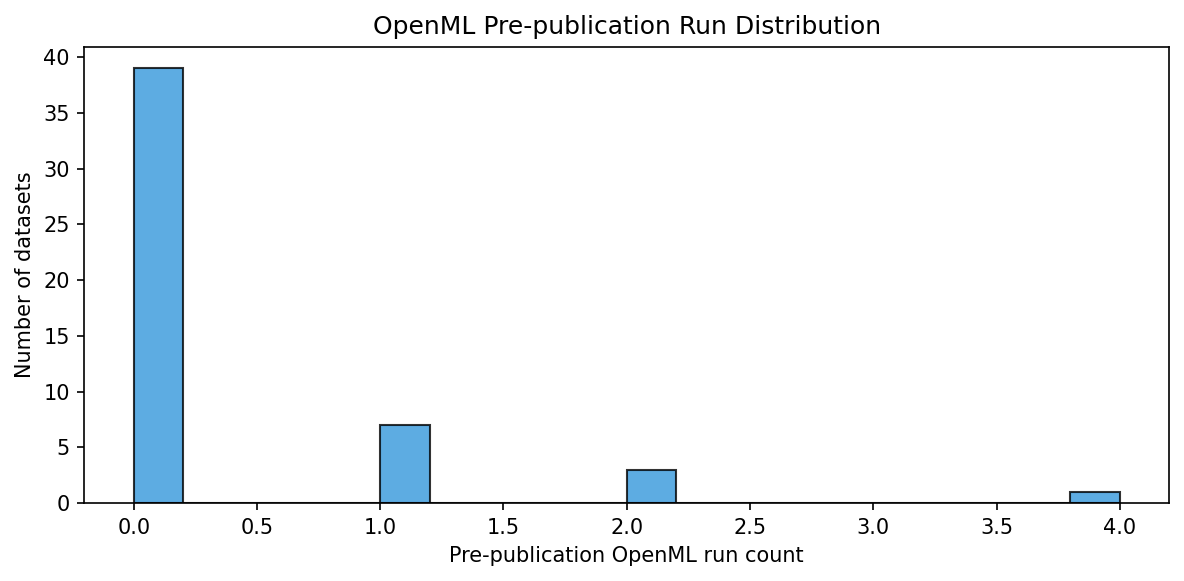
\includegraphics[width=0.9\linewidth]{figures/openml_run_dist.png}
\caption{Distribution of pre-publication run counts for 11 tabular/classical ML datasets in OpenML. All DL benchmarks have 0 OpenML entries.}
\label{fig:openml}
\end{figure}

The distribution is dominated by classical UCI datasets (adult, covertype, diabetes). MNIST appears with 1 OpenML entry. All DL benchmarks have 0 OpenML entries, confirming that OpenML cannot serve as a concentration proxy for the DL benchmarks that dominate Raff's corpus.

\subsection{Pipeline Validity}

\begin{table}[h]
\centering
\caption{Pipeline Activation Indicators}
\label{tab:activation}
\begin{tabular}{@{}lr@{}}
\toprule
Activation Indicator & Status \\
\midrule
HF Hub API reachable & $\checkmark$ PASS \\
OpenML API reachable & $\checkmark$ PASS \\
Raff CSV parseable (255 papers) & $\checkmark$ PASS \\
Temporal filter executable & $\checkmark$ PASS \\
\textbf{H-E1 gate (HF $\geq$50\% AND OpenML $\geq$70\%)} & $\times$ \textbf{FAIL} \\
\bottomrule
\end{tabular}
\end{table}

All 18 pipeline tests pass; runtime: 88.84 seconds. Raff corpus: 255 papers, 50.8\% reproducible. The gate fail is a genuine infrastructure finding, not an implementation defect.

\section{Discussion}
\label{sec:discussion}

\subsection{Key Findings and Their Implications}

\textbf{Finding 1: Both HF Hub and OpenML exhibit domain-temporal selection bias, not random coverage gaps.}

The 30\% HF coverage is concentrated in NLP benchmarks and small-scale image classification benchmarks (CIFAR-10, CIFAR-100, SVHN) that have been adopted by the HF ecosystem. The 22\% OpenML coverage is predominantly classical tabular datasets (iris, wine, adult, covertype, diabetes), with NLP benchmarks (IMDB, 20newsgroups) and MNIST also present. Large-scale DL vision (ImageNet, COCO, Pascal VOC, KITTI), speech (LibriSpeech, TIMIT, WSJ), and graph (Cora, Citeseer) datasets --- which dominate Raff's post-2012 deep learning papers --- are absent from both platforms.

\textbf{Finding 2: Papers With Code is the appropriate primary data source for a redesigned study.}

Papers With Code explicitly tracks paper-dataset linkages across all dataset domains and historical periods. Unlike HF Hub (NLP-centric) and OpenML (tabular-centric), PwC is designed for the paper-dataset-code linkage we require and covers Raff's corpus temporal period. The theoretical hypothesis --- documentation completeness and concentration predict reproducibility failure --- remains scientifically plausible and worth testing, but requires PwC as the data source.

\textbf{Finding 3: Retroactively-created HF cards are systematically thin.}

The 0.41 mean field-presence score reveals that even when a card exists, it may not contain the fields most relevant to the misuse mechanism. The \texttt{intended\_use} and \texttt{out\_of\_scope\_use} fields --- which directly encode scope boundaries --- are systematically absent from retroactively-created cards, consistent with the timing of the Datasheets schema publication.

\subsection{Limitations}

\textbf{Limitation 1: The original research question remains unanswered.} The central hypothesis --- do metadata signals predict reproducibility failure? --- is neither confirmed nor refuted. We report an infrastructure characterization. Running regression on 30\% IV1 coverage would produce biased, uninterpretable results; blocking was the correct decision.

\textbf{Limitation 2: H-E1 used canonical dataset names only.} Alternate name variants (e.g., ``uoft-cs/cifar10'') might recover additional HF cards. However, a scalable auditing pipeline requiring manual name variant curation defeats the purpose of automated auditing; the DL domain gap is structural in any case.

\textbf{Limitation 3: Results are specific to the Raff 2019 corpus.} Post-2019 papers with more NLP and HF-native datasets would show substantially higher HF coverage.

\textbf{Limitation 4: The theoretical mechanism remains empirically unverified.} The three-step causal chain (concentration $\to$ artifact accumulation; incompleteness $\to$ out-of-context application; joint effect $\to$ reproducibility failure) is theoretically grounded in \citet{DAm2021Underspecification} and \citet{Gebru2021Datasheets} but not yet empirically confirmed.

\subsection{Broader Impact}

Our infrastructure characterization directly benefits researchers planning HF+OpenML-based reproducibility auditing of pre-2018 ML literature. Without this characterization, such researchers would build pipelines that silently fail to represent 70--78\% of the target corpus. The validated pipeline components are immediately reusable for the redesigned PwC-based study.

A reflexivity note: the Datasheets schema we use to measure completeness was designed for new dataset creation, not retroactive annotation of 1990s benchmarks. Evaluating CIFAR-10 by whether its HF card contains an \texttt{out\_of\_scope\_use} field conflates absence-of-documentation with absence-of-concern-for-misuse. A redesigned study should address this temporal validity problem in the IV operationalization.

\section{Conclusion}
\label{sec:conclusion}

We began with a straightforward goal: measure how dataset documentation quality and benchmark concentration predict ML reproducibility failure, using HuggingFace Hub and OpenML as data sources. What we found instead was that the metadata infrastructure we assumed existed does not --- and that this absence follows a pattern that has implications for any researcher attempting programmatic reproducibility auditing of pre-2018 ML literature.

In this work, we designed and executed a systematic infrastructure feasibility study (H-E1) to determine whether HF Hub and OpenML can serve as data sources for a dataset-metadata-to-reproducibility-outcome regression study on Raff's 255-paper corpus. Our main contributions are:

\begin{enumerate}
  \item \textbf{The first empirical quantification of HF Hub and OpenML coverage for the Raff 2019 corpus:} HF Hub achieves 30\% dataset card coverage (15/50 datasets found, all NLP benchmarks); OpenML achieves 22\% pre-publication temporal coverage (11/50, all classical tabular). Both fall below the minimum thresholds required for valid regression analysis.

  \item \textbf{Characterization of the domain-temporal selection bias:} Coverage gaps precisely follow each platform's founding community. DL vision, speech, and graph datasets --- which dominate Raff's corpus --- are absent from both platforms.

  \item \textbf{Identification of Papers With Code as the appropriate primary data source:} Our findings provide a principled motivation for switching to Papers With Code API for a redesigned study.

  \item \textbf{A validated, reusable data acquisition pipeline:} RaffParser, HFCoverageChecker, OpenMLTemporalChecker, MetricsAggregator, and an 18-test suite are available for immediate reuse.
\end{enumerate}

\textbf{Future directions:} The highest-priority next experiment is a redesigned H-E1 using Papers With Code as primary API --- the most direct path to answering the original research question. Additional paths include systematic HF Hub name variant exploration (a lower-cost check of whether the 30\% figure is a lower bound) and extension to post-2019 corpora where HF coverage is substantially higher.

The infrastructure gap we discovered is both a limitation of this paper and a contribution to the field. Any researcher planning to use HF Hub and OpenML to study pre-2018 ML reproducibility should quantify coverage for their specific corpus before proceeding --- the structural domain biases in these platforms are invisible unless explicitly measured. We hope this work saves others from the same discovery at a later and more costly stage of their pipeline.


\bibliography{references}
\bibliographystyle{plainnat}

\newpage
\appendix
% Appendix placeholder — extend as needed


\end{document}
